\section{Results\label{sec:assess.results}}

The results presented in this section aim at answering the research questions defined in \Cref{sec:assess.intro}.
\Cref{fig:asssess.baseline} presents the performance of the global model without malicious participants to serve as a baseline to compare with.
The model displays relatively high performance on both datasets, \ie, above 0.9 for the accuracy, recall, and F1-score.
However, some classes are more challenging to detect than others.
The feeble representation of the ``Injection'' class in \texttt{cicids} (around 0.0017\%, see \Cref{tbl:assess.datasets}) prevents the model from learning from it, provoking this absence of evolution over time (see \Cref{fig:assess.baseline.cicids}).
The ``Infiltration'' class is more represented in the dataset (0.6108\%, approximately the same as the ``Brute Force'' and ``Bot'' classes), but remains difficult to learn because of its apparent similarity with benign traffic.
Consequently, it never exceeds a recall of 0.2.
The detection in \texttt{nb15} is better overall, with the exception of the ``Analysis'' and ``DoS'' classes that score below 0.9, although they are not the least represented classes in the dataset.

\begin{figure}
  \centering
  \begin{subfigure}{.45\linewidth}
    \centering
    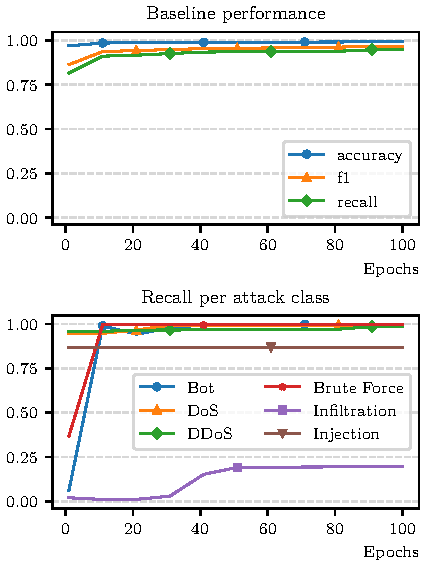
\includegraphics[width=\linewidth]{figures/cicids/baseline}
    \caption{
      CIC-CSE-IDS2018.
      \label{fig:assess.baseline.cicids}
    }
  \end{subfigure}
  \hfill
  \begin{subfigure}{.45\linewidth}
    \centering
    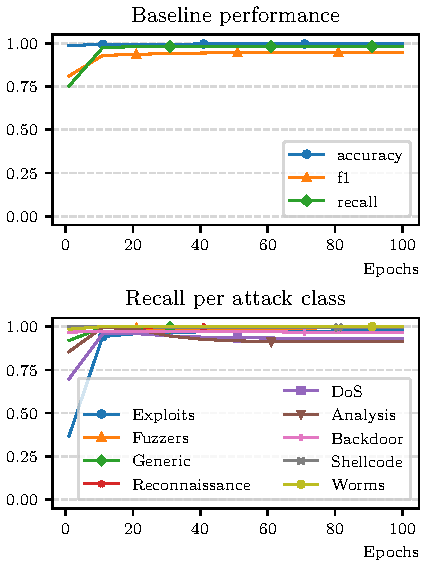
\includegraphics[width=\linewidth]{figures/nb15/baseline}
    \caption{
      UNSW-NB15.
      \label{fig:assess.baseline.nb15}
    }
  \end{subfigure}
  \caption{
    Performance of the global model without malicious participants.
    The accuracy, F1-score, and recall illustrate the performance that can be expected from the global model under the conditions selected for this study ($\mathcal{E}=10$, $\beta=512$).
    The recall of the six available attack classes shall serve as a reference for the \gls{rasr} of targeted attacks.
    \label{fig:assess.baseline}
  }
\end{figure}


% ------------------------------------------------------------------------------
% RQ1: PREDICTABILITY
% ------------------------------------------------------------------------------

\subsection{Impact Predictability\label{sec:results.predictability}}

\begin{figure}
  \centering
  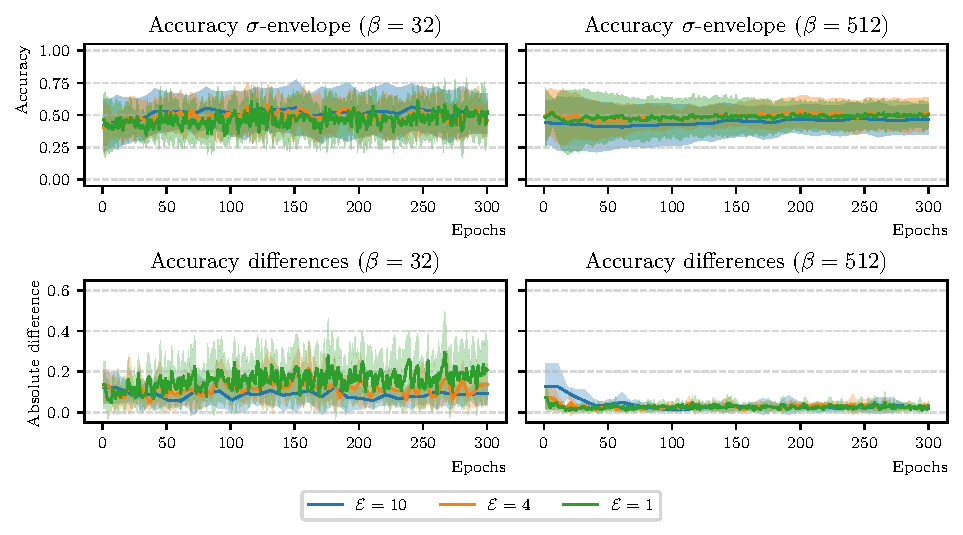
\includegraphics[width=\textwidth]{figures/cicids/predictability-all}
  \caption{
    Studying attack impact predictability over time, with 50\% attackers.
    The $x$-axis represents the number of local epochs.
    \Cref{fig:predictability.a} illustrates each seed's accuracy over time using a rolling mean with a window of 5. 
    \Cref{fig:predictability.b,fig:predictability.c} display envelopes with the mean values and the standard deviation of each experiment (over the ten seeds).
  }
  \label{fig:predictability}
  \phantomlabels{fig:predictability}{f}
\end{figure}